\documentclass[10.25pt,a4paper,oneside]{article}
\usepackage[a4paper,top=0.4in,left=0.4in,right=0.4in,bottom=0.4in]{geometry}
\usepackage{graphicx}
\usepackage{rotating}
\usepackage{hyperref}
\usepackage{setspace}
\usepackage{float}
\graphicspath{ {./images/} }
\pagenumbering{gobble}
\hypersetup{
	colorlinks=true,
	urlcolor=blue
}

\urlstyle{same}x

\begin{document}
{\setstretch{0.75}
\begin{center}
	\textsc{Group Project - 7CCSMGPR}
\end{center}
\begin{center}
	\hspace{0.5cm} Deadline Fighters \hspace{0.5 cm} Preliminary report - February 8, 2019
\end{center}

\section{Tools/Technology}
At first, we use GitHub for code hosting, GitHub is a hosting platform for open source and proprietary software projects. It benefits for the team work projects because every member in the team can modify code and pull requests.\\\\
We need to write documents use LaTex , Overleaf is an online LaTex editor that we make use of.\\\\
Before coding, we apply Mockingbot to design user interface and set standards for what the clients will look like.\\\\
For the server, we use Amazon S3, it is a simple cloud storage service. The main reason we use that instead of virtual machine is security, Amazon S3 uses the Advanced Encryption Standard for 256 bits, AES can quickly encrypt and decrypt in software and hardware. When accessKeyID and secretKeyID are exposed to public, the Amazon S3 will send an email to user.\\\\
For the desktop client, we plan to use JavaScript/html/CSS language and the editor is Visual studio code. The structure we use is electron because it integrates \emph{Chromium} and \emph{Node.js} very well together, interfaces and algorithms can be combined in an orderly manner.\\\\
For the mobile client, we use Java on Android studio platform. And for the database, we use Structured Query Language on MySQL.\\\\
At the step of web debugging, we decide to use Charles. Charles is a HTTP proxy server, when the users send requests to server or get responses from server, Charles can monitor all data.\\\\
Testing is a critical part, we decide to use unit test and we preliminarily use Mocha and Junit. Mocha is a testing tool for JavaScript, it is more flexible than other test frameworks. Junit is the most basic testing structure for Java, we should apply it to test mobile client.



\section{Team protocol}
The main method the team choose is that agile software developing, which means that the development is iterative and step-by-step. The project divided into several individual small projects and during developing these small projects, it goes through the requirement, plan, design, development, tests, deploy, review and then go to the next small project.\\\\
There are two types of meeting that the team will be held. The first type is held every week which all members should attend. During this meeting all the team members review the work done last week finding the potential problems and planning for the next week. It usually lasts for 1 hour.\\\\
The other type is held between 1-2 days and this is not for all members but between the members who have the same tasks assigned from last week. This meeting usually does not involve the decision making but the attendance review what they have do after last daily meeting. It lasts for not longer than 5 minutes.\\\\
All team members should push at least one commit every two days. Once a member pulls request on the git, at least 2 members should view changes and approve before it merges on the master branch of the repository. If some members request changes, the member who pulls request should be fixed or give a satisfactory explanation to these changes.


}
\begin{sidewaysfigure}
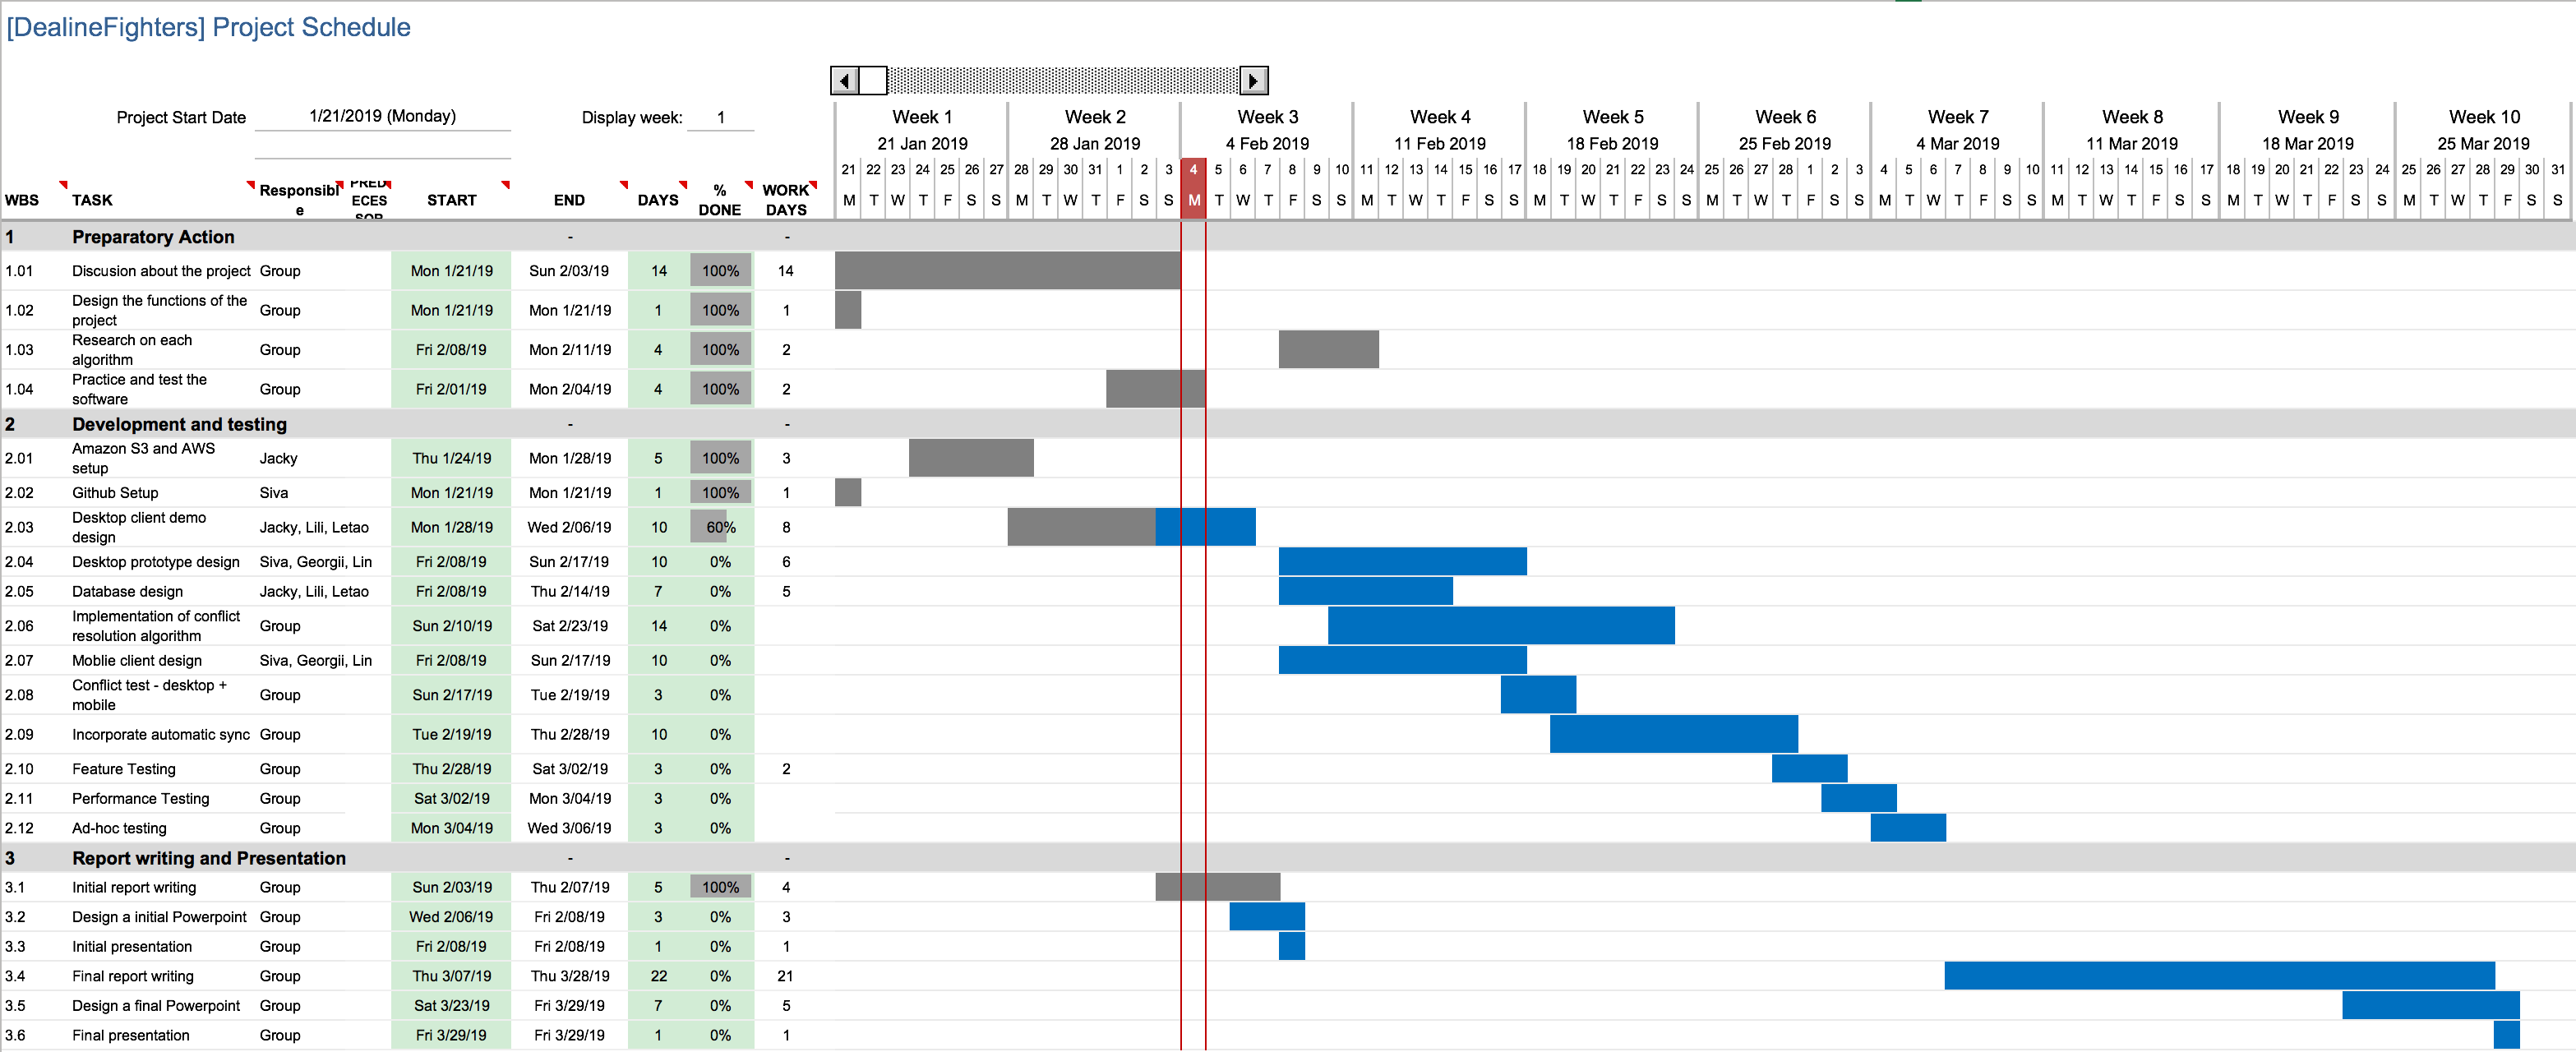
\includegraphics[scale=0.4]{Timeline_Ver_0}
\caption{This is Gantt chart which illustrates the plan of our group within 10 weeks.}
\end{sidewaysfigure}
\end{document}

